\documentclass[a4paper,10pt]{article}
\usepackage[utf8]{inputenc}
\usepackage[english]{babel}
\usepackage{indentfirst}
\usepackage{listings}
\usepackage{graphicx}
\usepackage{blindtext}
\usepackage{enumitem}
\usepackage{hyperref}
\usepackage[top=2.5cm,bottom=2.5cm,left=2.5cm,right=2.5cm]{geometry}
\pagestyle{headings}
\title{Mobile Embedded Group Project}
\author{Ilias Boulif, Jérémy Bricq, George Rusu}
\date{\today}
\begin{document}
\maketitle
\tableofcontents
\newpage
\section{Introduction}

The aim of this project is to propose an implementation of an IoT network using \textit{Rime} where the sensor data is published through an MQTT-Rime gateway to normal MQTT subscribers. To achieve that we have implemented as requested by the project's statement, a tree-based routing protocol using Rime and an MQTT-Rime gateway.

Firstly, we are going to explain the general structure of our system. Secondly, we are going to present and explain the different messages exchanged in a normal run. Then, we will explain the organization and the routing in our environment. We will speak briefly about our gateway and MQTT subscriber implementation. And finally, we will discuss about the optimizations we managed to implement.

The implementation source code of this project is available at \cite{github}.


\section{General structure of our system}
Our infrastructure is divided in 2 sides: over air network (root and sensors) and wired network. This infrastucture is illustrated in Figure \ref{fig:fig1}.

\begin{figure}[!htb]
\centering
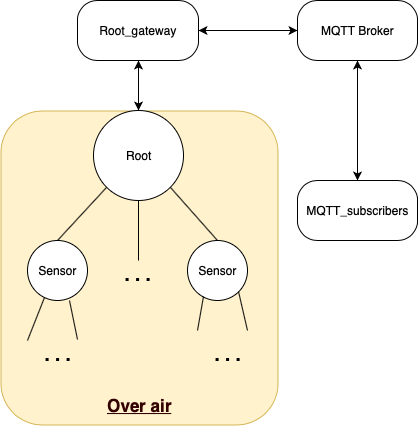
\includegraphics[scale=0.5]{./img/structure.png}
\caption{Representation of our structure}
\label{fig:fig1}
\end{figure}


The over air side (yellow part) is composed of one root node and a number of sensor nodes. When the sensor nodes have some collected data to publish, they will forward the information all the way up to the root. In order to accomplish that, there exists only one path from each sensor to the root. This is achieved by the fact that, each sensor chooses a parent according to its rank. In our system, the rank corresponds to the number of hops from the node to the root. Hence, when choosing a parent, each sensor will look for the parent with the lowest rank, in other words, with the shortest path to the root. \\

Once arrived at the top of the tree, the information is forwarded to the rime gateway which will publish all the sensor's information to the MQTT broker. The most important component is the root of the tree because he is responsible for the transmission of the data from the air network to the wired network. Once the data has been published in the broker, any MQTT subscriber can subscribe to topics in order to receive data of interest. \\

In our system, the nodes communicate together by sending different kind of messages that will be explained later in this document (see Section \ref{msgFormat}). Some of these messages are used to ensure a good working of the system. Indeed, the network is built as such to keep sending information up to the root even if a node is moved or deleted, this will be explained in the Section \ref{routing}. \\


Regarding the collection of data from the sensors by the root, there are two modes which describe the system's behaviour. The root receives some configuration messages, respectively the mode and the number of subscribers through the gateway.  He forwards the received configuration to the sensor nodes by the mean of the discovery and alive response packets, this will be explained in the Section \ref{gateway}. \\

Lastly, we will explain in Section \ref{subscriber} our MQTTsubscriber implementation which is basically a simple tool to subscribe to several or all topics in the broker.



\section{Message format}
\label{msgFormat}
In our implementation we have 3 packets structures. The node interprets the packet according to his type. We will explain each kind of packets and discuss the different types used by nodes to communicate between them.

\paragraph{Description of \textit{packet}}
\begin{enumerate}
\item Type : [DISCOVERY\_REQUEST, DISCOVERY\_RESPONSE, ALIVE\_REQUEST, ALIVE\_RESPONSE]
\item Rank : The rank of the transmitting node
\item Mode : The sent mode [DATA\_ON\_CHANGE, DATA\_PERIODICALLY] - by default, data periodically 
\item HaveSubscriber : Boolean that indicates if someone is subscribed to some topics
\end{enumerate}

\paragraph{Description of \textit{data\_packet} }
\begin{enumerate}
\item Type : [SENSOR\_DATA]
\item NodeSrc :  The source node transmitting the data
\item NodeRank : The rank of the node source
\item DataTemp : The temperature data
\item DataADXL : The accelerometer data
\end{enumerate}

\paragraph{Description of \textit{data\_packet\_aggregate} }
\begin{enumerate}
\item Type : [SENSOR\_DATA\_AGGREGATE]
\item numberPacket : The number of contained packets
\item packet1 :  The first packet
\item packet2 : The second packet
\end{enumerate}

\paragraph{DISCOVERY\_REQUEST}  When a node starts, his rank is equal to 0. The node will start to search for a network, and thus search for a parent to attach to. He will send in broadcast a discovery request to find a parent connected to that network. In order to have this work properly, we define that the root node will always have the same rank which is 1. Even when connected to a parent, the node will still keep sending discovery request in order to search the environment for a better parent, if there is one. The lowest the rank is (except a rank of 0), the nearest the node is to the root.

\paragraph{DISCOVERY\_RESPONSE} When a node receives a discovery request packet, he will reply with a discovery response containing his rank in unicast. The node that has made the request receive now the response, checks the received rank (parent+1) and if better than his cur according to the received rank, change or not assign the his rank the value of the rank of his parent + 1.

\paragraph{ALIVE\_REQUEST} Each node has to keep sending an alive request in order to know if his parent is still available in the network. After 4 alive requests without any response, the child considers that he has no parent. If he has no more parent, his rank return back to 0 and he has to research for a new one. 

\paragraph{ALIVE\_RESPONSE } When a node receives an alive request, he has to replies with an alive response to his child to validate his presence. Each alive response is accompanied with the rank of the parent. In this way, if the parent is disconnected from the network (rank = 0), the child can also put his rank to 0 and can disconnect. 

\paragraph{SENSOR\_DATA } A sensor data packet is a packet that contains some information collected by the sensor. This packet travels from his sensor to the subscribers by going forwarded by the nodes on the path to the root.

\paragraph{SENSOR\_DATA\_AGGREGATE } A sensor data aggregate packet is a packet that contains many sensors data packets in one. This packet will be explained in details in the Section \ref{opti} : Optimizations.





\section{Network organization and routing}
\label{routing}

\section{Gateway}
\label{gateway}
\section{MQTT-Subscriber}
\label{subscriber}
\section{Optimizations}
\label{opti}

\section{Conclusion}

\begin{thebibliography}{9}

\bibitem{github}
Github repository,
\textit{MobileEmbeddedComputing}, Available at :
\url{https://github.com/georgesrusu/MobileEmbeddedComputing}.


\end{thebibliography}
\end{document}